\documentclass[AMA,Times1COL]{WileyNJDv5} %STIX1COL,STIX2COL,STIXSMALL


\articletype{RESEARCH ARTICLE}%

\received{Date Month Year}
\revised{Date Month Year}
\accepted{Date Month Year}
\journal{Journal}
\volume{00}
\copyyear{2023}
\startpage{1}

\raggedbottom

% abbreviations
\newcommand{\ddd}{\,\mathrm{d}}
%%%%%%%%%%%
\newcommand{\by}{\boldsymbol{\mathrm{y}}}
\newcommand{\bY}{\boldsymbol{\mathrm{Y}}}
\newcommand{\bX}{\boldsymbol{\mathrm{X}}}
\newcommand{\bVp}{\boldsymbol{\mathrm{V}_0}}
%\newcommand{\bVpp}{\boldsymbol{\mathrm{V}_1}}
\newcommand{\bVpp}{\boldsymbol{\mathrm{V}^*}}
\newcommand{\bmp}{\boldsymbol{\mathrm{m}_0}}
%\newcommand{\bmpp}{\boldsymbol{\mathrm{m}_1}}
\newcommand{\bmpp}{\boldsymbol{\mathrm{m}^*}}
\newcommand{\bth}{\boldsymbol{\theta}}
\newcommand{\bxi}{\boldsymbol{\xi}}
\newcommand{\bWp}{\boldsymbol{\mathrm{W}_0}}
%\newcommand{\bWpp}{\boldsymbol{\mathrm{W}_1}}
\newcommand{\bWpp}{\boldsymbol{\mathrm{W}^*}}
\newcommand{\bC}{\boldsymbol{\mathrm{C}}}
%%%%%%%%%%%
\usepackage{bbm}
\usepackage{graphicx}
\usepackage{float} 
\usepackage{tikz}

\allowdisplaybreaks


\begin{document}

\title{Bayesian analysis for pretest-posttest binary outcomes with adaptive significance levels}
%Bayesian methodology to perform statistical analysis of pretest-posttest binary outcomes
\author[1]{Alejandra E. Pati\~no Hoyos}

\author[2]{Johnatan Cardona-Jim\'enez}

\author[2]{Tom\'as Rodr\'iguez Taborda}
%\author[3]{Author Three}

\authormark{PATI\~NO and CARDONA}
\titlemark{Bayesian analysis for pretest-posttest binary outcomes with adaptive  significance levels}

\address[1]{\orgdiv{Facultad de Ingenier\'ia}, \orgname{Instituci\'on Universitaria Pascual Bravo}, \orgaddress{\state{Medell\'in }, \country{Colombia}}}

\address[2]{\orgdiv{Facultad de Ciencias}, \orgname{Universidad Nacional de Colombia}, \orgaddress{\state{Medell\'in }, \country{Colombia}}}

% \address[3]{\orgdiv{Department Name}, \orgname{Institution Name}, \orgaddress{\state{State Name}, \country{Country Name}}}

\corres{Alejandra E. Pati\~no Hoyos, Departamento de Fundamentaci\'on, Instituci\'on Universitaria Pascual Bravo, 
73A - 226 Street 73, P.O. Box: 6564, Medellin, Colombia. \email{alejandra.patino@pascualbravo.edu.com}}

\presentaddress{This is sample for present address text this is sample for present address text.}

%\fundingInfo{Text}
%\JELinfo{ejlje}

\abstract[Abstract]{
% Counting outcomes are frequent in clinical and engineering studies. In frequentist statistical analysis, focus has centered on count data in independent samples scenarios. However, this approach doesn't address situations where pairs of measurements come from the same individual before and after treatment, like in pretest-posttest studies. Such designs call for paired sample tests. In the realm of count data, there's limited discussion within Bayesian statistical analysis for these setups. Here, we introduce a Bayesian statistical methodology for comparing paired samples in binary pretest-posttest scenarios. We establish a Bayesian probabilistic model for the inferential analysis of these paired samples, validate and refine this model through simulation, and ultimately apply our approach to a dataset extracted from specialized literature.


Count outcomes in longitudinal studies are common in clinical and engineering studies. In frequentist and Bayesian statistical analysis, methods such as mixed linear models allow the variability or correlation within individuals to be taken into account. However, in more straightforward scenarios, where only two stages of an experiment are observed (pre-treatment vs. post-treatment), there are only a few tools available, mainly for continuous outcomes. Thus, this work introduces a Bayesian statistical methodology for comparing paired samples in binary pretest-posttest scenarios. We establish a Bayesian probabilistic model for the inferential analysis of the unknown quantities, which is validated and refined through simulation analyses, and present an application to a dataset taken from the Television School and Family Smoking Prevention and Cessation Project (TVSFP) (Flay et al., 1995). The application of the Full Bayesian Significance Test (FBST) for precise hypothesis testing, along with the implementation of adaptive significance levels in the decision-making process, is included.}

\keywords{keyword1, keyword2, keyword3, keyword4}

\jnlcitation{\cname{%
\author{Taylor M.},
\author{Lauritzen P},
\author{Erath C}, and
\author{Mittal R}}.
\ctitle{On simplifying ‘incremental remap’-based transport schemes.} \cjournal{\it J Comput Phys.} \cvol{2021;00(00):1--18}.}


\maketitle

\renewcommand\thefootnote{}
\footnotetext{\textbf{Abbreviations:} ANA, anti-nuclear antibodies; APC, antigen-presenting cells; IRF, interferon regulatory factor.}

\renewcommand\thefootnote{\fnsymbol{footnote}}
\setcounter{footnote}{1}


\section{Introduction}

In longitudinal data, where subjects or elements are measured at different time points, the variability within these units of interest is vital in the statistical analyses commonly employed in these research studies. One of the most common tools statisticians and practitioners use in those contexts is the so-called linear mixed model (LMM). With that model, the investigator can relate one outcome with a group of predictors or covariates to either measure their impact on the response or predict new outcomes. To have successful modeling with LMMs, one has to have a good set of predictors and a significant sample size. Specifically, to obtain power levels of 80\% with a type I error of 0.05, large sample sizes are required for studies with a small number of repeated measures \cite{dang2008sample}. Thus, LMMs may not be the best option for studies with only two repeated measures and, much worse, with small sample sizes. In this sense, tools such as paired t-tests are commonly employed for studies with only two-time points and continuous responses \cite{diehr1995breaking, brookmeyer1998person, duncan2013self, chen2014comparison, forrester2015selecting, manfei2017differences, cowdery2019effectiveness, albassam2021testing}. One common approach for two repeated measures or pre-treatment vs. post-treatment studies with binary outcomes is the McNemar's test\cite{mcnemar1947note}. However, the test requires the same subjects to be observed before and after the treatment, which is not always the case in longitudinal studies. Additionally, the adequacy of the test is based on large sample sizes. Improvements, extensions, and alternatives from McNemar's test have been proposed in the literature \citep{ lu1995sample, morikawa19952chi, tango1998equivalence}. For instance, Tang and Tang\cite{tang2004exact} develop an exact test for two paired proportions with incomplete data. In a similar line of work, Tang et al. \cite{tang2005confidence} propose confidence intervals for comparing proportions in small-sample paired studies. Conversely, Tang et al. \cite{tang2010confidence} propose several asymptotic confidence intervals for the differences between proportions based on paired data. Taking advantage of treating proportion as special areas under receiver operating characteristic, Duan et al. \cite{duan2018novel} propose a non-parametric confidence interval for differences of proportions for correlated binary data. These methods cited so far have something in common: they are based on frequentist statistics, significant levels, and p-values. Regarding hypothesis testing, over the last two decades, concern has arisen about the misunderstanding and misuse of significant levels and p-value \cite{siegfried2010odds, cumming2013problem, siegfried2014make, nuzzo2014scientific, wasserstein2016asa}. From a Bayesian perspective, some proposals have emerged for alternatives to p-values \cite{johnson2013revised, pericchi2014adaptive, benjamin2016comment}.
In this work, we propose a Bayesian analysis for longitudinal data suitable for studies with few repeated measures related to binary outcomes. Specifically, we address the problem of two repeated measures. Along with that analysis, we implement fully Bayesian statistical test procedures for sharp and more general hypotheses testing scenarios with adaptive significant levels. To take into account the correlation due to the repeated measures, we employ the bivariate beta model as a prior distribution \cite{Olkin03, BIBBY2011} for the unknown probabilities of success. For the inferential procedures, the Bayesian approach is an attractive option for setting up counterparts for p-values, which are easier to interpret. For instance, if one has a hypothesis of the type $H_0: \theta\leq 0$, vs. $H_1: \theta>0$, for $0<\theta<1$, and $D$ is the information available to test the hypotheses under consideration, from a Bayesian perspective all is reduced to compute $P(H_0|D)=P(\theta\leq 0)$ and $P(H_1|D)=P(\theta> 0)$, and choose the most probable hypothesis. Computing the uncertainty or probability of a scientific hypothesis in that manner needs yet to be developed in a classic or frequentist context. On the other hand, for the sharp hypothesis of the type $H_0: \theta = 0$, vs. $H_1: \theta\neq 0$, one can employ the Full Bayesian Significant Test (FBST) \cite{PerSter-99, PerSteWech-08}. For both types of tests, we implement the option of adaptive significant levels following the ideas presented in \cite{Patino-23, GannonPer-2019, PeriPere-16}. In this context, adaptive significant levels mean that the thresholds to judge p-values are computed objectively from the tests and not set subjectively, as is usually the case in more traditional hypothesis testing procedures. In the next section, we introduce the probability models to describe the uncertainty of the unknown quantities, the Bayesian computations to update the prior information about the unknowns, and the inferential procedures and computations of the adaptive significant levels. In section \ref{sec1}, a simulation analysis is performed to evaluate and characterize the proposed methodology. In section \ref{sec2}, some applications regarding real data are presented. 






%In pre-post studies, the effect of an intervention is assessed by comparing a subject's outcomes before (pre) and after (post) receiving the intervention. In all these stages, each unit of analysis yields two outcomes from two different conditions. In this work, the primary interest lies in the difference between proportions when the observed variable is a binomial outcome at each stage. Since these measurements are correlated, statistical methods to compare independent samples cannot be applied. For continuous outcomes, the paired t-test is the standard statistical method in the frequentist approach for evaluating differences between means. However, the paired t-test does not apply to non-continuous variables such as binary and count outcomes. This work presents a Bayesian statistical method for comparing paired samples in binary pretest-posttest scenarios. The methodology includes the use of the Full Bayesian Significance Test (FBST) \cite{PerSter-99} for precise hypothesis testing and adaptive significance levels in the decision-making process.


%\begin{itemize}
%\justifying
%\setlength\itemsep{1em}
%    \item As well as continuous variables, count results arise quite frequently in both clinical research and engineering research.
%    \item The most adapted model for analyzing count data is the Poisson model. Other models that can be considered for modeling count data are binomial and negative binomial. 
 %   \item For example, the number of hospitalizations, the number of days of use and the number of packs of cigarettes smoked per day are popular count outcomes in mental health research.
    
 %      \item Studies that show paired results are also popular. For example, to evaluate new eye drops, one eye of a subject may be treated with the new eye drops and the other eye with a placebo drop. To evaluate skin cancer in drivers, skin cancer on the left arm can be compared to skin cancer on the right arm, since the left arm is more exposed to sunlight.
  %     \item In a pre-post study, the effect of an intervention is evaluated by comparing a subject's results before (pre) and after (post) receiving the intervention.

 %   \item In all of these studies, each unit of analysis has two outcomes arising from two different conditions. Interest focuses on the difference between the means of the two results in the case in which the measure of interest is continuous, or focuses on the difference in proportions when the variable is the result of counting some characteristic of interest.
%    \item For continuous outcomes, the paired t test is the standard statistical method from the frequentist approach to evaluate differences between means. However, the paired t test does not apply to non-continuous variables such as binary and count outcomes.
%\end{itemize}

\section{Methodology}\label{sec1a}

Let $y_{ij}$, for $i = 1,..., n_j$, be binary random variables related to the $i$-th individual or sample unit at a time $j$, with $j = 1,2$. For example, in a medical pre-post study, these paired results correspond to the pre and post-treatment evaluation. These measurements are performed on the same group of subjects; therefore, statistical methods to compare independent samples cannot be applied. In that way, one can define the following new random variables: $X_{j}=\sum _{i} y_{ij}$, where $X_{j}\vert \theta_j \sim \text{bin} (n_j,\theta_j)$ with $\theta_j$ being the success probability at the stage $j$. Given $\boldsymbol{\theta}=(\theta_1,\theta_2)$, $X_{1}$ and $X_{2}$ are conditionally independent, thus, their joint distribution is such that $(X_{1}, X_{2}) \vert \boldsymbol{\theta} \sim \text{bin} (n_1,\theta_1) \times \text{bin} (n_2,\theta_2)$. The unconditional dependency between $X_{1}$ and $X_{2}$ is introduced through the bivariate distribution of $(\theta_1,\theta_2)$. That estructure is grapically described in Figure \ref{fig:diagrama_muestras}. As a prior distribution for $\boldsymbol{\theta}$, we propose the three-parameter bivariate beta model proposed by Olkin and Liu \cite{Olkin03}, also called the two-dimensional beta distribution. That distribution has a
density given by  
%, which allows for positive correlation

% Let $X_{ij}$, $i = 1,..., n$ be random variables that represent the count measurements for the $i$-th individual or sample unit at a time $j$, with $j = 1,2$. For example, in a medical pre-post study, this paired results correspond to the pre and post-treatment evaluation. This measurements are correlated, then, statistical methods to compare independent samples cannot be applied. In that way, for each individual, we have a bivariate vector $\bX_i = (X_{i1}, X_{i2})^{\top}$, where $X_{ij}\vert \theta_j \sim \text{bin} (n_j,\theta_j)$. Given, $\boldsymbol{\theta}=(\theta_1,\theta_2)$, $X_{i1}$ and $X_{i2}$ are conditionally independent, thus, their joint distribution is such that $\bX_i \vert \boldsymbol{\theta} \sim \text{bin} (n_1,\theta_1) \times \text{bin} (n_2,\theta_2)$. The unconditional
% correlation between $X_{i2}$ and $X_{i2}$ is introduced through the bivariate distribution of $(\theta_1,\theta_2)$. We propose then as prior use of the $3$ parameter bivariate beta model proposed by Olkin and Liu \cite{Olkin03} allowed for positive correlation, called also the \textbf{two-dimensional beta distribution} that has a density given by 

\begin{equation}\label{prior}
f(\boldsymbol{\theta})=\dfrac{\Gamma(\alpha)}{\Gamma(\alpha_1)\Gamma(\alpha_2)\Gamma(\alpha_0)} \, \dfrac{\theta_1^{\alpha_1-1} (1-\theta_1)^{\alpha_2+\alpha_0-1}\, \theta_2^{\alpha_2-1} (1-\theta_2)^{\alpha_1+\alpha_0-1}}{(1-\theta_1\theta_2)^{\alpha}},
\end{equation}

for $0 < \theta_1 < 1$, $0 < \theta_2 < 1$, and $\alpha = \alpha_1 + \alpha_2 + \alpha_0$.

\begin{figure}[ht]
    \centering
    \begin{tikzpicture}[scale=1.5]
        \node (f) at (0,0) {\(f(\theta_1, \theta_2)\)};
        \node (theta1) at (-2,-2) {\(\theta_1\)};
        \node (theta2) at (2,-2) {\(\theta_2\)};
        \node (X1) at (-2,-4) {\(X_1\)};
        \node (X2) at (2,-4) {\(X_2\)};
        \draw[->] (f) -- (theta1);
        \draw[->] (f) -- (theta2);
        \draw[->] (theta1) -- (X1);
        \draw[->] (theta2) -- (X2);
        \draw[-] (theta1) -- (theta2);
    \end{tikzpicture}
    \caption{The samples \(X_1\) and \(X_2\) are conditionally independent given \(\boldsymbol{\theta} = (\theta_1, \theta_2)\), where the uncertainty of both \(\theta_1\) and \(\theta_2\) are jointly modeled by \(f(\boldsymbol{\theta})\)=\(f(\theta_1, \theta_2)\).}
    \label{fig:diagrama_muestras}
\end{figure}
% for the bivariate $\bX_i$. 
% Given, $\boldsymbol{\theta}=(\theta_1,\theta_2)$, $X_{i1}$ and $X_{i2}$ are conditionally independent and follow a binomial distribution $X_{ij}\vert \theta_j \sim \text{bin} (n_j,\theta_j)$. Then, we have the joint distribution $\bX_i \vert \boldsymbol{\theta} \sim \text{bin} (n_1,\theta_1) \times \text{bin} (n_2,\theta_2)$. 

% follows that 

% where $X_{i1}$ and $X_{i2}$ are said to be conditionally independent given $\boldsymbol{\theta}=(\theta_1,\theta_2)$ and , 

% then follows the joint distribution 

% \begin{equation*}
% f(x_{i1}, x_{i2} \vert \boldsymbol{\theta})={n_1 \choose x_{i1}} \, {\theta_{1}}^{x_{i1}} \,{(1-\theta_{1})} ^{n_1-x_{i1}}.
% \end{equation*}

% Consider a sample of $n$ individuals indexed by $i$, and let $y_{i1}$ and $y_{i2}$ be the paired outcomes of the $i$-th individual. For example, in a medical pre-post study, the paired results correspond to the pre and post-treatment evaluation. This two measurements are correlated, then, statistical methods to compare independent samples cannot be applied.

\vspace{2mm}
% The marginal distribution of $\bX_i$ called the \textbf{two-dimensional beta binomial distribution} is introduced by Bibby and V\ae th \cite{BIBBY2011} and has a probability mass function given by
% \begin{align}\label{margx}
% f(x_{i1}, x_{i2})&=\int_{
% [1,0]^2}f_{\bX_i \vert \boldsymbol{\theta}}(x_i \vert \boldsymbol{\theta} )\, f(\boldsymbol{\theta})\, d\boldsymbol{\theta}\nonumber\\[3pt]
% &= {n_1 \choose x_{i1}} {n_2 \choose x_{i2}} \dfrac{\Gamma(\alpha)}{\Gamma(\alpha_0)\Gamma(\alpha_1)\Gamma(\alpha_2)} \, \dfrac{\Gamma(x_{i1}+\alpha_1)\,  \Gamma(n_1-x_{i1}+\alpha-\alpha_1)}{\Gamma(n_1
% +\alpha)} \nonumber\\[3pt]
% &\times \dfrac{\Gamma(x_{i2}+\alpha_2) \,  \Gamma(n_2-x_{i2}+\alpha-\alpha_2)}{\Gamma(n_2
% +\alpha)} \nonumber\\
% &\times {}_3 F_2(\alpha,x_{i1}+\alpha_1, x_{i2}+\alpha_2; n_1+\alpha, n_2+\alpha;1)
% \end{align}

%for $x_{i1}=0,1, \dots n_1$ and $x_{i2}=0,1, \dots n_2$. \newline
%where $\bX\in\boldsymbol{\Omega}$
The marginal distribution of $\bX=(X_{1}, X_{2})$, called the \textbf{two-dimensional beta binomial distribution}, is introduced by Bibby and V{\ae}th \cite{BIBBY2011} and has the probability mass function given by
\begin{align}\label{margx}
f(\bX)&=\int_{
[1,0]^2}f_{\bX \vert \boldsymbol{\theta}}(x_{1}, x_{2} \vert \boldsymbol{\theta} )\, f(\boldsymbol{\theta})\, d\boldsymbol{\theta}\nonumber\\[3pt]
&= {n_1 \choose x_{1}} {n_2 \choose x_{2}} \dfrac{\Gamma(\alpha)}{\Gamma(\alpha_0)\Gamma(\alpha_1)\Gamma(\alpha_2)} \, \dfrac{\Gamma(x_{1}+\alpha_1)\,  \Gamma(n_1-x_{1}+\alpha-\alpha_1)}{\Gamma(n_1
+\alpha)} \nonumber\\[3pt]
&\times \dfrac{\Gamma(x_{2}+\alpha_2) \,  \Gamma(n_2-x_{2}+\alpha-\alpha_2)}{\Gamma(n_2
+\alpha)} \nonumber\\
&\times {}_3 F_2(\alpha,x_{1}+\alpha_1, x_{2}+\alpha_2; n_1+\alpha, n_2+\alpha;1)
\end{align}

for $x_{1}=0,1, \dots n_1$ and $x_{2}=0,1, \dots n_2$. Here ${}_3 F_2$ is a generalized hypergeometric function. The generalized hypergeometric function in
(\ref{margx}) is well-defined as $\alpha_0$ is assumed to be positive. Thus, the posterior distribution of $\boldsymbol{\theta}$ in closed form is given by\newpage

% \begin{align}\label{posti}
% f(\theta_1, \theta_2 \vert x_{i1}, x_{i2})&=
% \dfrac{\Gamma(n_1+\alpha)}{\Gamma(x_{i1}+\alpha_1)\Gamma(n_1-x_{i1}+\alpha-\alpha_1)} \, \dfrac{\Gamma(n_2+\alpha)}{\Gamma(x_{i2}+\alpha_2)\Gamma(n_2-x_{i2}+\alpha-\alpha_2)} \nonumber\\[3.5pt]
% &\times \dfrac{\theta_1^{\alpha_1+x_{i1}-1} (1-\theta_1)^{\alpha_2+\alpha_0+n_1-x_{i1}-1} \, \theta_2^{\alpha_2+x_{i2}-1} (1-\theta_2)^{\alpha_1+\alpha_0+n_2-x_{i2}-1}}{(1-\theta_1\theta_2)^{\alpha}}\nonumber\\[3pt]
% &\times  \left[{}_3 F_2(\alpha,x_{i1}+\alpha_1, x_{i2}+\alpha_2; n_1+\alpha, n_2+\alpha;1)\right]^{-1}
% \end{align}

%Thus, the Bayesian posterior distribution of $\bth$ is given by


\begin{align}\label{posti}
f(\boldsymbol{\theta} \vert \bX)=\frac{f(\bX\vert \boldsymbol{\theta})f(\boldsymbol{\theta})}{f(\bX)}&=
\dfrac{\Gamma(n_1+\alpha)}{\Gamma(x_{1}+\alpha_1)\Gamma(n_1-x_{1}+\alpha-\alpha_1)} \, \dfrac{\Gamma(n_2+\alpha)}{\Gamma(x_{2}+\alpha_2)\Gamma(n_2-x_{2}+\alpha-\alpha_2)} \nonumber\\[3.5pt]
&\times \dfrac{\theta_1^{\alpha_1+x_{1}-1} (1-\theta_1)^{\alpha_2+\alpha_0+n_1-x_{1}-1} \, \theta_2^{\alpha_2+x_{2}-1} (1-\theta_2)^{\alpha_1+\alpha_0+n_2-x_{2}-1}}{(1-\theta_1\theta_2)^{\alpha}}\nonumber\\[3pt]
&\times  \left[{}_3 F_2(\alpha,x_{1}+\alpha_1, x_{2}+\alpha_2; n_1+\alpha, n_2+\alpha;1)\right]^{-1}
\end{align}





\subsection{Non-informative bivariate beta prior distribution}\label{secKL}

An important concern in Bayesian analysis is the level of information brought by the prior distribution. Some researchers are reluctant to bring different sources of information rather than the data itself in their statistical analysis. These researchers prefer the use of "objective" or non-informative priors distribution. Thus, for the case of the prior distribution (\ref{prior}), we define a non-informative or vague prior distribution through a Kullback-Liebler (KL) divergence. The process to obtain such distribution is the describe as follows:\newline
A measure of the distance or divergence between the densities $p(\boldsymbol{\theta})$ and $q(\boldsymbol{\theta})$ is defined by

\begin{equation}\label{KL}
 D\left[p(\boldsymbol{\theta});q(\boldsymbol{\theta})\right]=\int p(\boldsymbol{\theta})\,log\left(\frac{p(\boldsymbol{\theta})}{q(\boldsymbol{\theta})}\right)d\boldsymbol{\theta}= E\left[ log\left(\frac{p(\boldsymbol{\theta})}{q(\boldsymbol{\theta})}\right)\right]. 
\end{equation}

Smaller values for $D$ indicate closer distributions in the KL sense. In the limit, when $p = q$, the divergence is null. This distance could be used to evaluate the quality of an approximation $q(\theta)$ for $p(\theta)$ \cite{Gamerman2014}. Thus, in order to approximate the bivariate beta to a non-informative prior, the KL divergence was minimized by taking $q(\theta_1,\theta_2)$ as in (\ref{prior}) and 
\begin{equation}\label{unifB}
p(\theta_1,\theta_2)=\dfrac{\Gamma(\lambda_1,\beta_1)}{\Gamma(\lambda_1)\Gamma(\beta_1)} \, \theta_1^{\lambda_1-1} (1-\theta_1)^{\beta_1-1} \, \times \, \dfrac{\Gamma(\lambda_2,\beta_2)}{\Gamma(\lambda_2)\Gamma(\beta_2)} \, \theta_2^{\lambda_2-1} (1-\theta_2)^{\beta_2-1}, 
\end{equation}
\vspace{1em}

with $\lambda_1=\beta_1=\lambda_2=\beta_2=1$.
\vspace{1em} 

That is, we find through a minimization process the $\alpha_0$, $\alpha_1$ and $\alpha_2$ values that minimize the divergence in (\ref{KL}), and in that way, we find the hyperparameters that approximate the bivariate beta distribution in (\ref{prior}) to a uniform prior distribution. Given there is no closed-form solution for the integral in (\ref{KL}), the measure of the distance $D$ can be approximated via Monte Carlo integration:

\begin{equation*}\label{KL3}
 D\left[p(\boldsymbol{\theta});q(\boldsymbol{\theta})\right]= 
 E\left[ log\left(\frac{p(\boldsymbol{\theta})}{q(\boldsymbol{\theta})}\right)\right] \approx \frac{1}{M}\sum\limits_{j=1}^{M}  log\left(\frac{p(\boldsymbol{\theta_j})}{q(\boldsymbol{\theta_j})}\right), 
\end{equation*}

where $M$ values of $\boldsymbol{\theta}$ are draw from the bivariate uniform distribution defined in (\ref{unifB}).
%On the other hand, the measure of the distance $D$ in \eqref{KL} can be approximately determined via Monte Carlo simulation. Define

%\begin{equation*}
%g(\boldsymbol{\theta})=log\left(\frac{p(\boldsymbol{\theta})}{q(\boldsymbol{\theta})}\right)d\boldsymbol{\theta},
%\end{equation*}

%and $h(\boldsymbol{\theta})$ as a two-dimensional uniform distribution. We can write,




%Then, generating $M$ samples of $\boldsymbol{\theta}$ from $h(\boldsymbol{\theta})$, we can approximate the measure of the distance $D$ in \eqref{KL} by Monte Carlo simulation through the expression

%\begin{equation*}\label{KL3}
 %D\left[p(\boldsymbol{\theta});q(\boldsymbol{\theta})\right]= 
% E\left[ \frac{g(\boldsymbol{\theta})}{h(\boldsymbol{\theta})}\right] \approx \frac{1}{M}\sum\limits_{j=1}^{M} \frac{g(\boldsymbol{\theta_i})}{h(\boldsymbol{\theta_i})}. 
%\end{equation*}

\subsection{Full Bayesian Significance Test  (FBST)}

The \emph{Full Bayesian Significance Test}  (FBST) was introduced by Pereira and Stern \cite{PerSter-99} as a method to evaluate precise or ``sharp"  hypotheses. These hypotheses involve subsets of $\boldsymbol{\Theta}$ (parameter space) that have fewer dimensions compared to the entire parameter space. Consequently, these subsets have a null Lebesgue measure. The FBST determines the strength of evidence in support of the hypothesis $\text{\textbf{H}}$ by considering the complement of the posterior probability of the Highest Posterior Density (HPD) region. This HPD region is tangential to the set defining the null hypothesis. With the FBST, the authors introduce the \textit{e}-value as an evidence index in favor of the null hypothesis (\textbf{H}). 

% The formal definition of FBST is as follows \cite{MadPer-05}:

% Consider a standard parametric statistical model, i.e., for an integer $m$, $\theta \in \Theta \subset \mathbb{R}^m$ is the parameter, $g(\theta)$ a prior probability density over $\Theta$, $x_0$ is the observed data, and $L_{x_0}(\theta)$ is the likelihood generated by $x_0$. After data $x_0$ have been observed, the posterior probability density for $\theta$ given $x_0$ is denoted by
% $f(\theta\vert x_0)\propto L_{x_0}(\theta)\,g(\theta)$.

% Consider a null hypothesis ${\text{\textbf{H}}: \theta \in \Theta_\text{\textbf{H}}}$ (sharp hypothesis, i.e., $dim(\Theta_\text{\textbf{H}})<dim(\Theta)$). The tangential set to $\text{\textbf{H}}$ is given by
% \begin{equation*}
% T_{x_0}=\left\lbrace \theta \in \Theta: f(\theta\vert x_0)>\underset{\text{\textbf{H}}}{\operatorname{sup}}f(\theta\vert x_0) \right\rbrace.
% \end{equation*}
% The measure of evidence (e-value) in favor of $\text{\textbf{H}}$ is defined as the posterior probability of the complement of $T_{x_0}$, that is, 
% \begin{equation*}
% ev\left(\text{\textbf{H}};x_0\right)=1-P(\theta \in T_{x_0}\vert x_0)=1-\int_{T_{x_0}}f(\theta\vert x_0)\, d\theta.  
% \end{equation*}

% The \textbf{FBST} is the procedure that rejects $\text{\textbf{H}}$ whenever $ev\left(\text{\textbf{H}};x_0\right)$ is small (\cite{PerSteWech-08}).

%\label{defFBST}

In the context of our problem, we are interested in testing the hypotheses
\begin{align*}
\text{\textbf{H}}&: \theta_1=\theta_2\\
\text{\textbf{A}}&: \theta_1 \neq \theta_2.
\end{align*}

Let $\boldsymbol{\Theta}_\text{\textbf{H}}$ and $\boldsymbol{\Theta}_\text{\textbf{A}}$ be the partition of the parameter space defined by the competing hypotheses \textbf{H} and \textbf{A}. % consider a null hypothesis ${\text{\textbf{H}}: \boldsymbol{\theta} \in \boldsymbol{\Theta}_\text{\textbf{H}}}$ and the alternative hypothesis ${\text{\textbf{A}}: \boldsymbol{\theta} \in \boldsymbol{\Theta}_\text{\textbf{A}}}$. 
The tangential set to $\text{\textbf{H}}$ is given by
%\begin{small}
\begin{equation}
T_{x_{1},x_{2}}=\left\lbrace (\theta_1,\theta_2)\in \boldsymbol{\Theta}: f(\theta_1,\theta_2\vert x_{1},x_{2})>\underset{\text{\textbf{H}}}{\operatorname{sup}}f(\theta_1,\theta_2\vert x_{1},x_{2}) \right\rbrace.
\end{equation}
%\end{small}
The measure of evidence ($e$-value) in favor of $\text{\textbf{H}}$ is defined as the $T_{x_{10},x_{20}}$ posterior probability complement, that is, 
%\begin{small}
\begin{align}\label{ev}
ev\left(\text{\textbf{H}};x_{1},x_{2}\right)&=1-P((\theta_1,\theta_2) \in T_{x_{1},x_{2}}\vert x_{1},x_{2})\nonumber\\
&=1- \int_{} \int_{T_{x_{1},x_{2}}}f(\theta_1,\theta_2\vert x_{1},x_{2})\, d\theta_1 d\theta_2.  
\end{align}
%\end{small}
The \textbf{FBST} is the procedure that rejects $\text{\textbf{H}}$ whenever the $ev\left(\text{\textbf{H}};x_{1},x_{2}\right)$ is small \cite{PerSteWech-08}. Thus, the natural question would be: How
small does the value have to be? That is an unsolved question in Bayesian analysis and frequentist statistics with p-values.
The standard approach is to define an arbitrary cutoff, usually 0.05. In the next section, a method to define objective cutoffs as function of the sample size and the dimension of $\boldsymbol{\Theta}$ is presented.

\subsection{Adaptive cutoff values for evidence in the FBST}

In the context of regression linear models, Patiño et al. \cite{Patino-23} propose to establish a cutoff value $k^*$ for the $ev\left(\text{\textbf{H}};x_{1},x_{2}\right)$ in the FBST as a function of the sample size $n$ and the dimensionality of the parameter space $d$, i.e., $ k^*= k^*(n,d)$ with $k^*\in [0,1]$. Such $k^*$ is designed to minimize the linear combination of the averaged type-I ($\alpha_{\varphi_{e}}$) and type-II ($\beta_{\varphi_{e}}$) error probabilities: $a\alpha_{\varphi_{e}}+b\beta_{\varphi_{e}}$, with $a, b \in \mathbb{R}$. The $a$ and $b$ values denote the comparative importance of the two error types or, alternatively, the relative prior preferences toward the competing hypotheses. This approach is more general than the one usually adopted in frenquentist statistics, where type-I error probability is fixed arbitrarily and from that value type-II error is minimized. To describe the procedure, consider the test
% \begin{equation}
% \varphi_{e}(x)= \left\{ \begin{array}{l}  0 \quad if \quad ev\left(\text{\textbf{H}};x\right)> k\\ \\ 1 \quad if \quad ev\left(\text{\textbf{H}};x\right)\leq 
% k.  \end{array} \right.\;
% \end{equation}

\begin{equation*}
\varphi_{e}(x_{1},x_{2})= \left\{ \begin{array}{l}  0 \quad if \quad ev\left(\text{\textbf{H}};x_{1},x_{2}\right)> k\\ \\ 1 \quad if \quad ev\left(\text{\textbf{H}};x_{1},x_{2}\right)\leq 
k.  \end{array} \right.\;
\end{equation*}When $\varphi_{e}(x_{1},x_{2})=0$, there is evidence in favor of $\text{\textbf{H}}$ or $\varphi_{e}(x_{1},x_{2})=1$, there is evidence in favor of $\text{\textbf{A}}=\boldsymbol{\Theta}\setminus \text{\textbf{H}}$.  Thus, for $(X_{1}, X_{2}) \in \boldsymbol{\Omega}_{x}$, where $\boldsymbol{\Omega}_{x}$ is the sample space, the power function is given by
% \begin{eqnarray}
% \pi_{\varphi_{e}}(\theta)=P\left(\lbrace X \in \Omega:\varphi_{e}(X)=1 \rbrace\vert \,\theta\right)=P\left( \left\lbrace X \in \Omega: ev\left(\text{\textbf{H}};X\right)\leq 
% k\right\rbrace \Bigm| \theta\right),
% \end{eqnarray}

\begin{align}
\pi_{\varphi_{e}}(\boldsymbol{\theta})&=P\left( \left\lbrace (X_{1}, X_{2}) \in \boldsymbol{\Omega}_x:\varphi_{e}(X_{1}, X_{2})=1 \right\rbrace \Bigm| \boldsymbol{\theta}\right),\nonumber\\ 
&=P\left( \left\lbrace (X_{1}, X_{2}) \in \boldsymbol{\Omega}_x: ev\left(\text{\textbf{H}};X_{1}, X_{2}\right)\leq 
k\right\rbrace \Bigm| \boldsymbol{\theta}\right),\\
&=\int f_{{\bX \vert \boldsymbol{\theta}}}(x_{1}, x_{2}\vert \boldsymbol{\theta}) \, \mathbbm{1} \left(ev\left(\text{\textbf{H}};x_{1}, x_{2} \right)\leq 
k\right)d\boldsymbol{x},\nonumber
\end{align}where $f_{{\bX \vert \boldsymbol{\theta}}}(x_{1}, x_{2}\vert \boldsymbol{\theta})$ is the likelihood function and $\mathbbm{1}(\cdot)$ is the indicator function. A more appropriate notation would be $(X_{1}(n_1), X_{2}(n_2)) \in \boldsymbol{\Omega}_x$, to emphasize the dependence on the sample sizes $n_1$ and $n_2$, however, we keep $(X_{1}, X_{2}) \in \boldsymbol{\Omega}_x$ for simplicity. Thus, the averaged error probabilities II and I are respectively

\begin{align}\label{erro2}
\beta_{\varphi_{e}} &=  E_\theta\left[ 1-\pi_{\varphi_{e}}(\theta)\vert \text{\textbf{A}}\right]\nonumber\\
   & =  E_\theta\left[P\left(\left\lbrace (X_{1}, X_{2})  \in \boldsymbol{\Omega}:\varphi_{e}(X_{1}, X_{2}) =0\right\rbrace\Bigm|\boldsymbol{\theta}\right) \Bigm\vert \text{\textbf{A}}\right]\nonumber\\
   & = E_\theta\left[P\left(\left\lbrace (X_{1}, X_{2})  \in \boldsymbol{\Omega}:\left(ev\left(\text{\textbf{H}};x_{1}, x_{2} \right)> 
k\right)\right\rbrace\Bigm|\boldsymbol{\theta}\right) \Bigm\vert \text{\textbf{A}}\right]\nonumber\\
  & = E_\theta\left[P\left(\left\lbrace (X_{1}, X_{2})  \in \boldsymbol{\Omega}:\left(ev\left(\text{\textbf{H}};x_{1}, x_{2} \right)> 
k\right)\right\rbrace\Bigm|\boldsymbol{\theta}\right) \Bigm\vert \boldsymbol{\Theta}\setminus \text{\textbf{H}}\right]\nonumber\\
& = E_\theta\left[P\left(\left\lbrace (X_{1}, X_{2})  \in \boldsymbol{\Omega}:\left(ev\left(\text{\textbf{H}};x_{1}, x_{2} \right)> 
k\right)\right\rbrace\Bigm|\boldsymbol{\theta}\right) \Bigm\vert \boldsymbol{\Theta} - \{\theta_1=\theta_2\} \right]\nonumber\\
& = \int_{ \boldsymbol{\theta} \in \boldsymbol{\Theta} - \{\theta_1=\theta_2\}}\int_{(x_{1}, x_{2}) \in \boldsymbol{\Omega}} f_{{\bX \vert \boldsymbol{\theta}}}(x_{1}, x_{2}\vert \boldsymbol{\theta}) \, \mathbbm{1} \left(ev\left(\text{\textbf{H}};x_{1}, x_{2} \right)> 
k\right) \, f(\boldsymbol{\theta}) \, d\boldsymbol{x} \,d\boldsymbol{\theta},\nonumber\\
& = \int_{ \boldsymbol{\theta} \in \boldsymbol{\Theta} }\int_{(x_{1}, x_{2}) \in \boldsymbol{\Omega}} f_{{\bX \vert \boldsymbol{\theta}}}(x_{1}, x_{2}\vert \boldsymbol{\theta}) \, \mathbbm{1} \left(ev\left(\text{\textbf{H}};x_{1}, x_{2} \right)> 
k\right) \, f(\boldsymbol{\theta}) \, d\boldsymbol{x} \,d\boldsymbol{\theta},
\end{align}

and

\begin{align}\label{erro1}
\alpha_{\varphi_{e}} = & E_\theta\left[ \pi_{\varphi_{e}}(\theta)\vert \text{\textbf{H}}\right], \nonumber\\ 
 =&E_\theta\left[  P\left(\left\lbrace (X_{1}, X_{2})  \in \boldsymbol{\Omega}:\varphi_{e}(X_{1}, X_{2}) =1 \right\rbrace\Bigm|\boldsymbol{\theta}\right)\Bigm|\text{\textbf{H}}\right],\nonumber\\ 
=&E_\theta\left[ P\left( \left\lbrace (X_{1}, X_{2}) \in \boldsymbol{\Omega}: ev\left(\text{\textbf{H}};X_{1}, X_{2} \right)\leq 
k\right\rbrace \Bigm|\boldsymbol{\theta}\right)\Bigm|\text{\textbf{H}}\right],\nonumber\\
% =&\int_{0}^{1}\int_{(x_{1}, x_{2}) \in \boldsymbol{\Omega}} f_{\bX \vert \theta}(x_{1}, x_{2}\vert \theta) \, \mathbbm{1} \left(ev\left(\text{\textbf{H}};x_{1}, x_{2} \right)\leq 
% k\right) \, d\boldsymbol{x} \,d\theta
=&\oint_{\textbf{H}} \pi_{\varphi_{e}}(\boldsymbol{\theta}) \,f_{\textbf{H}}(\boldsymbol{\theta}) \,d\boldsymbol{\theta}, 
\end{align}

where $f_{\textbf{H}}(\boldsymbol{\theta})$ is the prior density under $\text{\textbf{H}}$ computed as

\begin{align}\label{priorH}
f_\textbf{H}(\theta_1,\theta_2)
&=\dfrac{f(\theta_1,\theta_2)\, \mathbbm{1}(\theta_1=\theta_2)}{\oint_{\textbf{H}} f(\theta_1,\theta_2) \, \, d\theta_1\,d\theta_2}.
\end{align}The prior $f_{\textbf{H}}(\boldsymbol{\theta})$ is graphically illustrated in Figure \ref{fig:mi_imagen}, and the computation of the line integral in (\ref{priorH}) is presented in the appendix section.
\begin{figure}[b]
    \centering
    \includegraphics[width=0.5\textwidth]{Figures/line_integral_corregido.png}  
    \caption{The prior $f(\boldsymbol{\theta})$ is sliced along the line $\theta_1 = \theta_2$. The moved section exposes the prior on the lower-dimensional subset where $\theta_1 = \theta_2$.}
    \label{fig:mi_imagen} 
\end{figure}The evidence in \eqref{ev} and the averaged error probabilities in \eqref{erro1} and \eqref{erro2} are computed via Monte Carlo integration. Therefore, the adaptive cutoff value $k^{*}$ for $ev\left(\text{\textbf{H}};x_{1},x_{2}\right)$ is the value of $k$ that minimizes $a\alpha_{\varphi_{e}}+b\beta_{\varphi_{e}}$, for fixed $a, b>0$. 
\vspace{3pt}
%Finally, consider %$\varphi_{e}^{*}(x)$ as 
%the test %such that
%\begin{equation}
%\varphi_{e}^{*}(x)= \left\{ \begin{array}{l}  0 \quad if \quad ev\left(\text{\textbf{H}};x_{1},x_{2}\right)> k^{*}\\ \\ 1 \quad if \quad ev\left(\text{\textbf{H}};x_{1},x_{2}\right)\leq 
%k^{*}.  \end{array} \right.\;
%\end{equation}
%\vspace{15pt}
Thus, the optimal averaged error probabilities that depend on the sample information are given by %the errors in \ref{erro1} and \ref{erro2} evaluated in such $k^{*}$
\begin{equation}
\alpha_{\varphi_{e}^{*}}^{*}= P\left(\left\lbrace (X_{1}, X_{2})  \in \boldsymbol{\Omega}:\varphi_{e}^{*}(X_{1}, X_{2}) =1 \right\rbrace\Bigm|\text{\textbf{H}}\right)=P\left( \left\lbrace (X_{1}, X_{2}) \in \boldsymbol{\Omega}: ev\left(\text{\textbf{H}};X_{1}, X_{2} \right)\leq 
k^{*}\right\rbrace \Bigm|\text{\textbf{H}}\right)
\end{equation}
\begin{equation}
\beta_{\varphi_{e}^{*}}^{*}=P\left(\left\lbrace (X_{1}, X_{2})  \in \boldsymbol{\Omega}:\varphi_{e}^{*}(X_{1}, X_{2}) =0\right\rbrace\Bigm|\text{\textbf{A}}\right)=P\left(  \left\lbrace (X_{1}, X_{2}) \in \boldsymbol{\Omega}: ev\left(\text{\textbf{H}};X_{1}, X_{2} \right)> 
k^{*}\right\rbrace \Bigm| \text{\textbf{A}}\right).
\end{equation}

The first concern that arises from (\ref{erro2}) and (\ref{erro1}) to anyone aware of the mechanisms behind any Bayesian analysis is the total
dependence on the prior distribution and the absence of the actual information from the experiment or data analyzed. Thus, the
computation of the averaged type-I ($\alpha_{\varphi_{e}}$) and type-II ($\beta_{\varphi_{e}}$) error probabilities depends not only on the sample sizes but also on the form
of the prior distribution. We propose one way to ease such a fair concern. In order to take an "objective" path of analysis, we define the posterior averaged type-I ($\alpha_{\varphi_{e}}$) and type-II ($\beta_{\varphi_{e}}$) error probabilities as:
\newpage

\begin{align}\label{erro2_2}
\beta_{\varphi_{e}} &= \int_{ \boldsymbol{\theta} \in \boldsymbol{\Theta} - \{\theta_1=\theta_2\}}\int_{(x_{1}, x_{2}) \in \boldsymbol{\Omega}} f_{{\bX \vert \boldsymbol{\theta}}}(x_{1}, x_{2}\vert \boldsymbol{\theta}) \, \mathbbm{1} \left(ev\left(\text{\textbf{H}};x_{1}, x_{2} \right)> 
k\right) \, f(\boldsymbol{\theta}|\boldsymbol{x}_{obs}) \, d\boldsymbol{x} \,d\boldsymbol{\theta},\nonumber\\
& = \int_{ \boldsymbol{\theta} \in \boldsymbol{\Theta} }\int_{(x_{1}, x_{2}) \in \boldsymbol{\Omega}} f_{{\bX \vert \boldsymbol{\theta}}}(x_{1}, x_{2}\vert \boldsymbol{\theta}) \, \mathbbm{1} \left(ev\left(\text{\textbf{H}};x_{1}, x_{2} \right)> 
k\right) \, f(\boldsymbol{\theta}|\boldsymbol{x}_{obs}) \, d\boldsymbol{x} \,d\boldsymbol{\theta},
\end{align}
and
\begin{align}\label{erro1_2}
\alpha_{\varphi_{e}} = &\oint_{\textbf{H}} \pi_{\varphi_{e}}(\boldsymbol{\theta}) \,f_{\textbf{H}}(\boldsymbol{\theta}|\boldsymbol{x}_{obs}) \,d\boldsymbol{\theta}. 
\end{align}

Some differences about working with (\ref{erro2_2}) and (\ref{erro1_2}) instead of (\ref{erro1}) and (\ref{erro2}) are that one is using an updated version of the prior distribution with the information from the particular experiment analyzed and that the $\beta_{\varphi_{e}}$ and $\alpha_{\varphi_{e}}$ are unique for any particular experiment. In contrast, working with (\ref{erro1}) and (\ref{erro2}), the values of $\beta_{\varphi_{e}}$ and $\alpha_{\varphi_{e}}$ are general for a fixed sample size regardless of the information of the actual experiment studied.


\section{Simulation Study}\label{sec1}


This section presents a simulation study to assess inferential procedures related to model (\ref{posti}): point and interval estimation and hypothesis testing. We employed non-informative and informative prior distributions to frame the Bayesian analysis performed in this simulation study. The non-informative prior is chosen to approximate a state of ignorance regarding the actual parameter values. In this case, the prior is derived based on the Kullback-Leibler divergence, as described in section \ref{secKL}. This allows us to obtain a prior that minimally informs the posterior distribution given the data. In addition to the non-informative prior, we designed the simulation to explore two scenarios using an informative prior based on specific values assigned to the parameters $\theta_1$ and $\theta_2$: one scenario where there is a conflict between the generated data and the prior distribution and another where there is no conflict. Conflict here means that there is a disagreement between the data and the prior information.


The informative prior was generated by deliberately selecting hyperparameter values of $\alpha_1 = \alpha_2 = \alpha_0=10$. In scenarios where $\theta_1 = \theta_2 = 0.1$, the informative prior introduces a degree of conflict with the data. Conversely, when set at $\theta_1 = \theta_2 = 0.5$, this prior aligns well with the data generation mechanism. Thus, the selection of the informative prior serves as a critical factor in assessing the robustness of the Bayesian inference process under varying degrees of compatibility with the observed data.

%This chapter presents a simulation study aimed at estimating the parameters $\boldsymbol{\theta}=(\theta_1,\theta_2)$ through Bayesian inference from posterior in \eqref{posti}. Specifically, we utilize Markov Chain Monte Carlo (MCMC) methods to derive estimates based on the posterior distribution's mode and mean, considering how these estimates vary as a function of the sample size ( $n_1=n_2$).



Once the priors were defined, we model the data as originating from two independent binomial distributions defined by the parameters $n_1$ and $n_2$ for $\theta_1$ and $\theta_2$, respectively. The probability of success in each trial is specified as
$\bX_i \vert \boldsymbol{\theta} \sim \text{bin}(n_1, \theta_1) \times \text{bin}(n_2, \theta_2)$. Figures \ref{prior1}, \ref{prior2}, an \ref{prior3} illustrate the priors and the respective posteriors obtained by the described procedure for a fixed value of $n_1=n_2=20$. As it was said, this study employed a simulation procedure to explore the behavior of the Bayesian estimates of $\theta_1$ and $\theta_2$ as the sample size varies. Specifically, the simulation was repeated $100$ times for each configuration of $n_1=n_2$, focusing on the influence of different types of prior distributions. Each iteration of the simulation involved the following steps:

\begin{itemize}
\setlength\itemsep{1em}
    \item \textbf{Data Generation:} For each of the $100$ simulations, random samples of size $n_1=n_2$ were drawn from the respective binomial distributions with the success probabilities set to $0.1$ and $0.5$ when it was applicable.
    \item \textbf{MCMC Estimation:} We implemented an MCMC algorithm, specifically designed to sample from the posterior distribution of the parameters $\boldsymbol{\theta}=(\theta_1,\theta_2)$. The algorithm was initialized with both the non-informative prior and the two informative priors, allowing for a comparative analysis of parameter estimates based on prior beliefs.
    \item \textbf{Posterior Analysis:} Post MCMC, we computed the mode (the maximum a posteriori estimate) and the mean (the expected a posteriori estimate) of the posterior distributions for both parameters. This analysis was conducted for varying values of $n_1=n_2$ , providing comparative insights into how sample size and prior information influence parameter estimation. Finally, to assess the uncertainty around our parameter estimates, we computed $95\%$ credible intervals for both $\theta_1$ and $\theta_2$. These intervals were derived from the resulting posterior samples, utilizing the quantiles at the 2.5th and 97.5th percentiles as the boundaries for each parameter’s credible interval.
\end{itemize}

\begin{figure}[h!]
\setlength{\tabcolsep}{15pt}
\begin{tabular}{cc}
    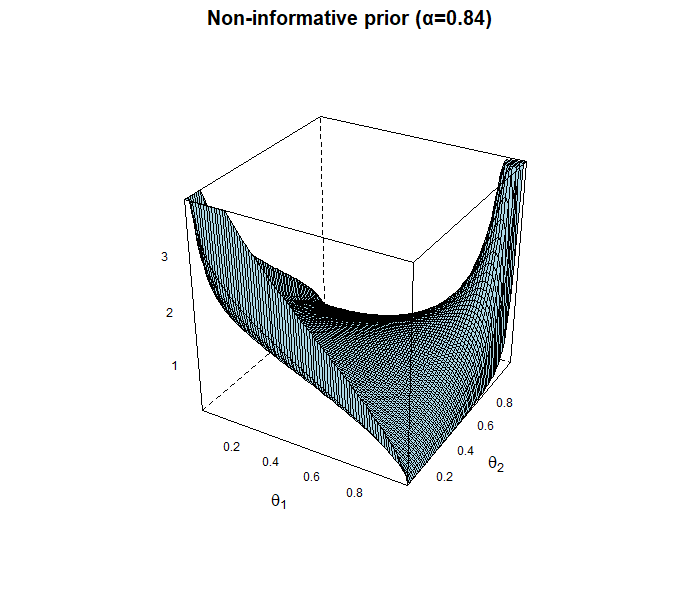
\includegraphics[scale=0.38]{Figures/prior_noinf.png} &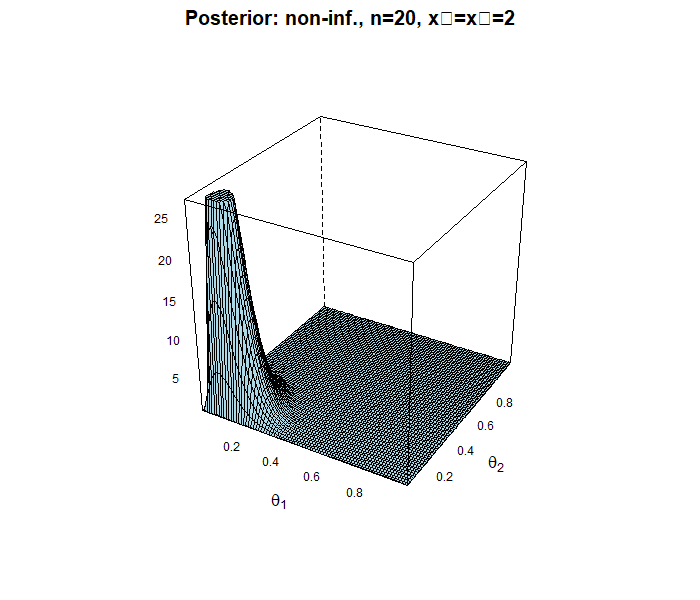
\includegraphics[scale=0.38]{Figures/post_noinf_n20_t0.1.png} \\
     \scriptsize (a) &  \scriptsize (b) 
 \end{tabular}

\caption{ (a) Non-informative prior approximated by Kullback-Liebler divergence. (b) Posterior distribution of $\bth$, taking  $\bX_i \vert \boldsymbol{\theta} \sim \text{bin} (n_1,\theta_1) \times \text{bin} (n_2,\theta_2)$ with $n_1=n_2=20$ and $\theta_1=\theta_2=0.1$.}
\label{prior1}
\end{figure}

\begin{figure}[h!]
\setlength{\tabcolsep}{5pt}
\begin{tabular}{cc}
    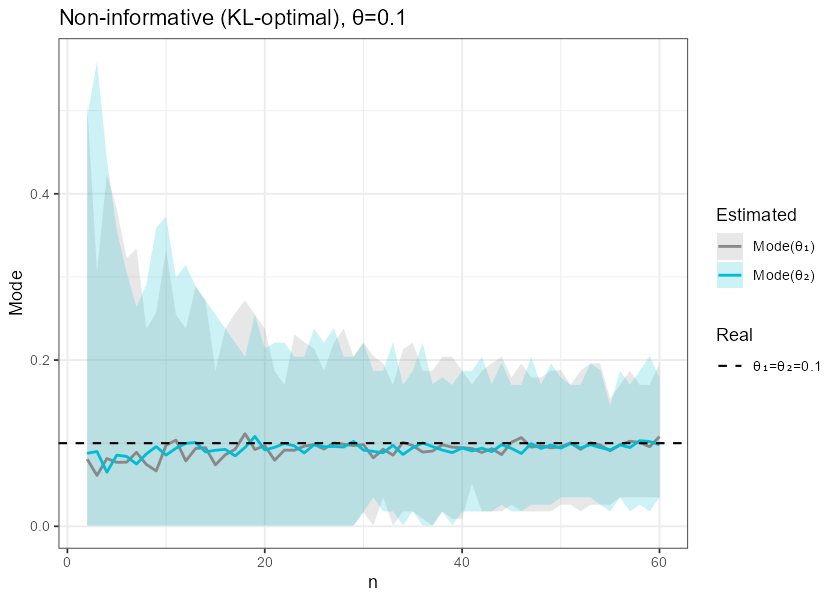
\includegraphics[scale=0.46]{Figures/mode_noinf_100_stan.png} &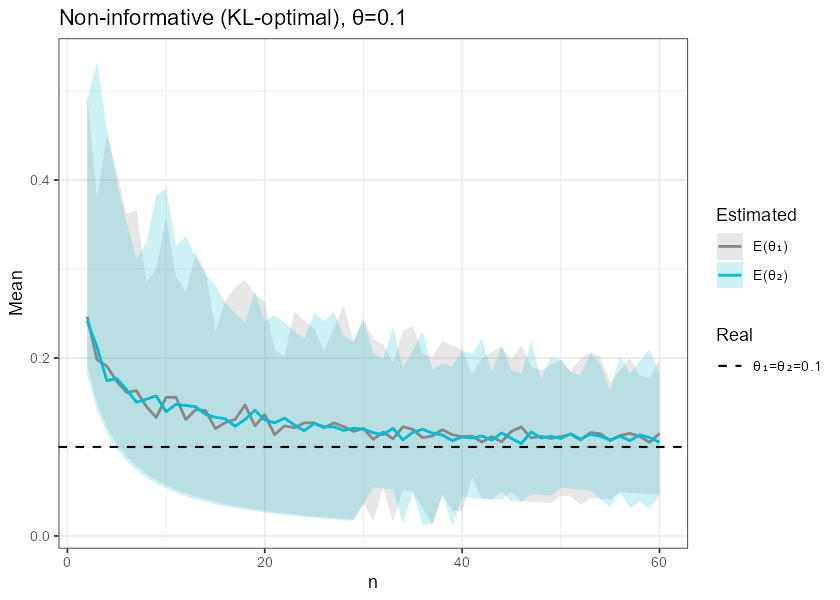
\includegraphics[scale=0.46]{Figures/mean_noinf_100_stan.png} \\
     \scriptsize (a) &  \scriptsize (b) 
 \end{tabular}

\caption{MCMC estimation of $\bth$ by the mode (a)  and the mean (b) of the posterior distribution as a function of $n=n_1=n_2$, taking  $\bX_i \vert \boldsymbol{\theta} \sim \text{bin} (n_1,\theta_1) \times \text{bin} (n_2,\theta_2)$ with $\theta_1=\theta_2=0.1$.}
\label{sim1}
\end{figure}

\begin{figure}[h!]
\setlength{\tabcolsep}{15pt}
\begin{tabular}{cc}
    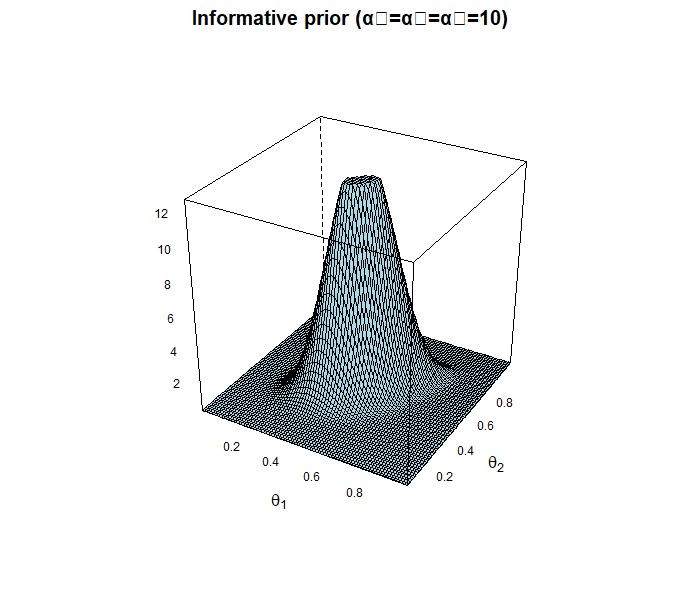
\includegraphics[scale=0.38]{Figures/prior_inf_Confl.png} &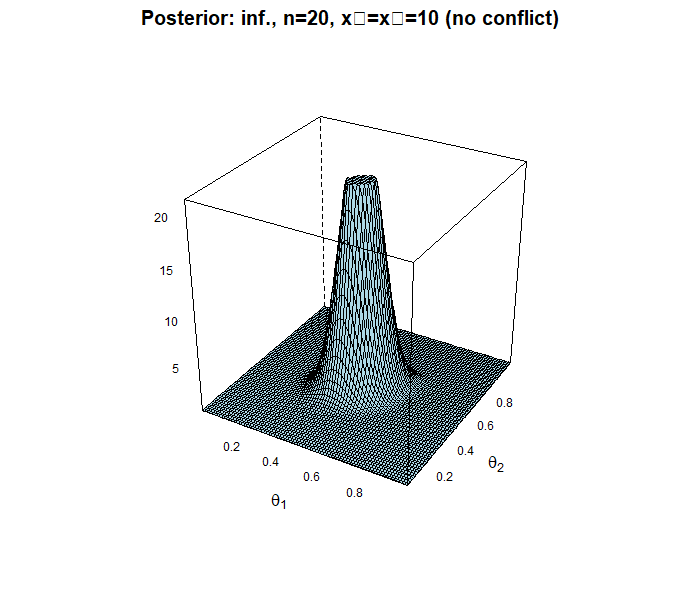
\includegraphics[scale=0.38]{Figures/post_inf_n20_t0.5.png} \\
     \scriptsize (a) &  \scriptsize (b) 
 \end{tabular}

\caption{(a) Informative prior with $\alpha_1 = \alpha_2 = \alpha_0=10$. (b) Posterior distribution of $\bth$, taking  $\bX_i \vert \boldsymbol{\theta} \sim \text{bin} (n_1,\theta_1) \times \text{bin} (n_2,\theta_2)$ with $n_1=n_2=20$ and $\theta_1=\theta_2=0.5$ (Prior-Data No Conflict).}
\label{prior2}
\end{figure}

\begin{figure}[h!]
\setlength{\tabcolsep}{5pt}
\begin{tabular}{cc}
    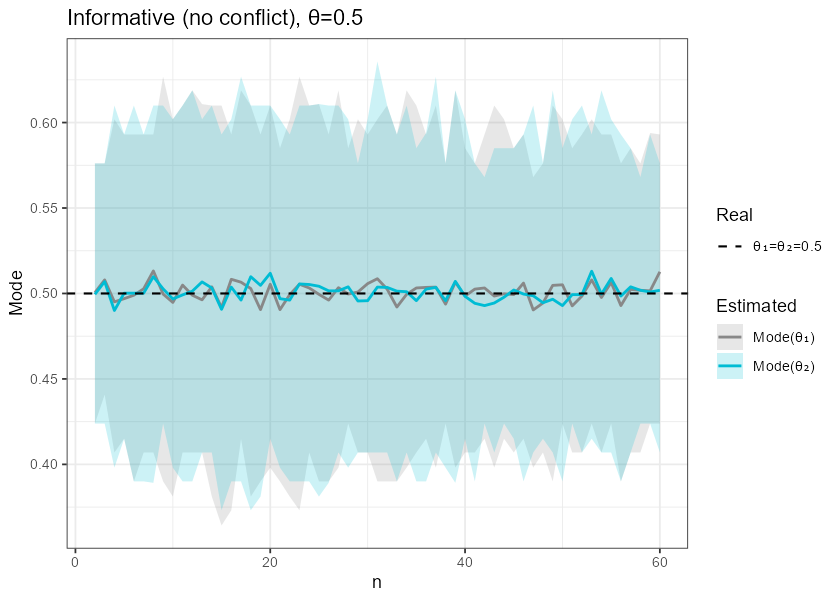
\includegraphics[scale=0.46]{Figures/mode_inf_100_NoConfl_stan.png} &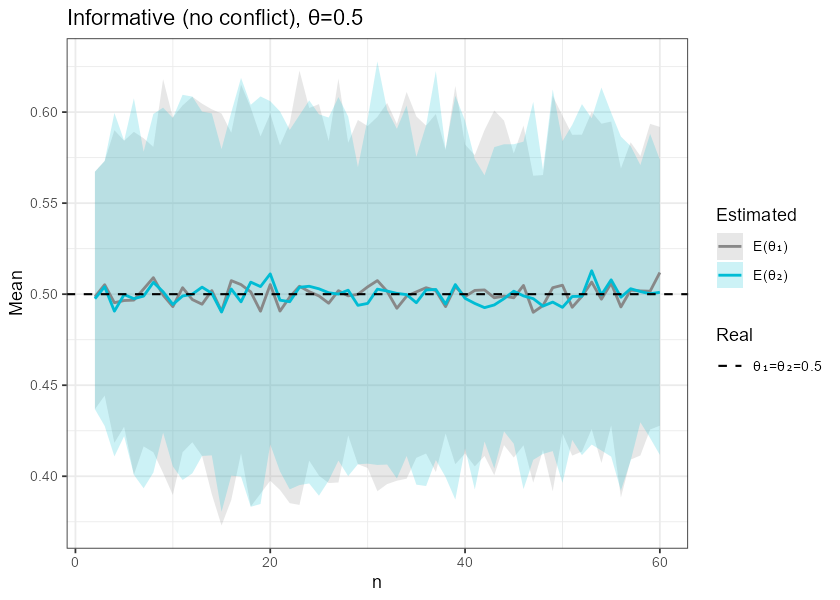
\includegraphics[scale=0.46]{Figures/mean_inf_100_NoConfl_stan.png} \\
     \scriptsize (a) &  \scriptsize (b) 
 \end{tabular}

\caption{MCMC estimation of $\bth$ by the mode (a)  and the mean (b) of the posterior distribution as a function of $n=n_1=n_2$, taking  $\bX_i \vert \boldsymbol{\theta} \sim \text{bin} (n_1,\theta_1) \times \text{bin} (n_2,\theta_2)$ with $\theta_1=\theta_2=0.5$ (Prior-Data No Conflict).}
\label{sim2}
\end{figure}

\begin{figure}[h!]
\setlength{\tabcolsep}{15pt}
\begin{tabular}{cc}
    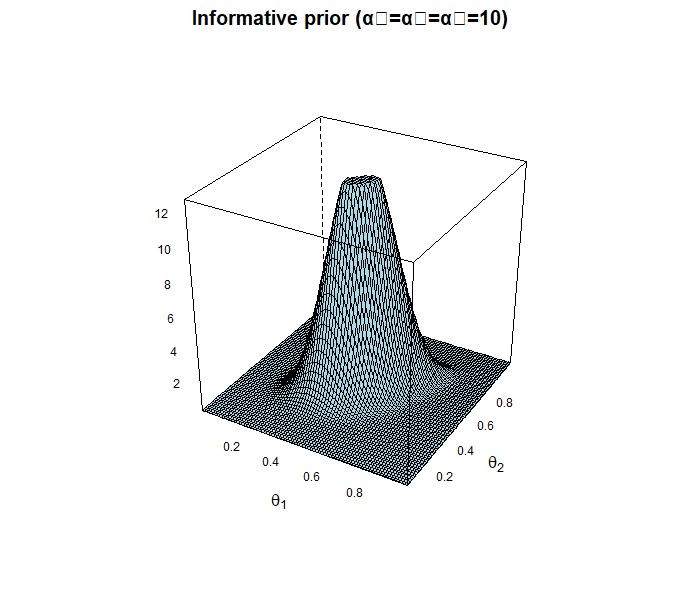
\includegraphics[scale=0.38]{Figures/prior_inf_Confl.png} &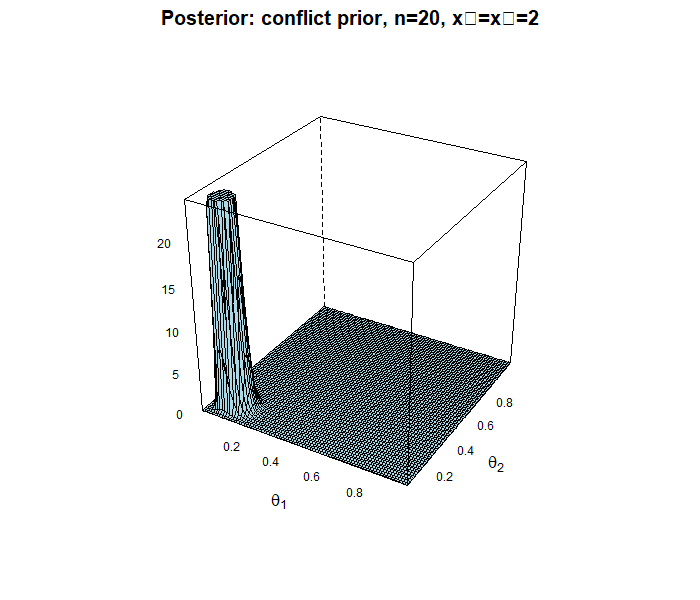
\includegraphics[scale=0.38]{Figures/post_inf_n20_t0.1_Confl.png} \\
     \scriptsize (a) &  \scriptsize (b) 
 \end{tabular}

\caption{(a) Informative prior with $\alpha_1 = \alpha_2 = \alpha_0=10$. (b) Posterior distribution of $\bth$, taking  $\bX_i \vert \boldsymbol{\theta} \sim \text{bin} (n_1,\theta_1) \times \text{bin} (n_2,\theta_2)$ with $n_1=n_2=20$ and $\theta_1=\theta_2=0.1$ (Prior-Data Conflict).}
\label{prior3}
\end{figure}

\begin{figure}[h!]
\setlength{\tabcolsep}{5pt}
\begin{tabular}{cc}
    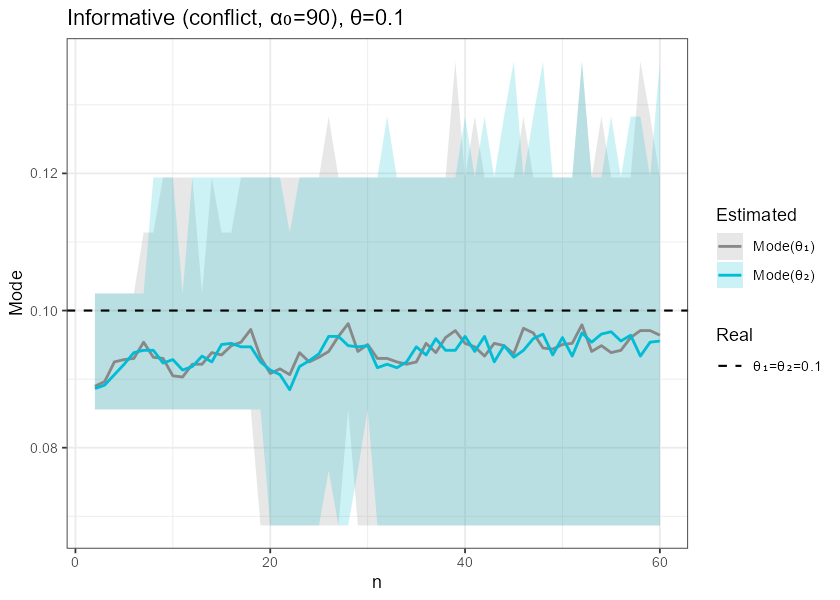
\includegraphics[scale=0.46]{Figures/mode_inf_100_Confl_stan.png} &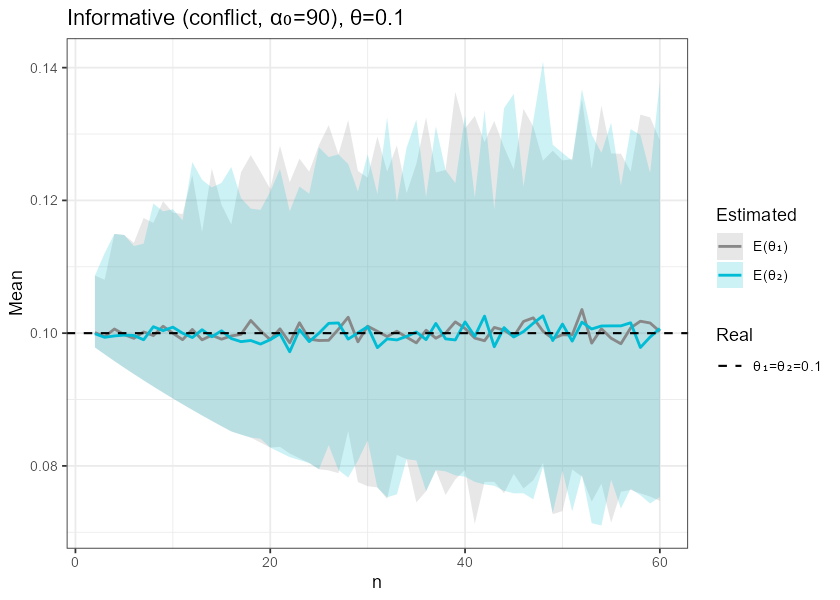
\includegraphics[scale=0.46]{Figures/mean_inf_100_Confl_stan.png} \\
     \scriptsize (a) &  \scriptsize (b) 
 \end{tabular}

\caption{MCMC estimation of $\bth$ by the mode (a)  and the mean (b) of the posterior distribution as a function of $n=n_1=n_2$, taking  $\bX_i \vert \boldsymbol{\theta} \sim \text{bin} (n_1,\theta_1) \times \text{bin} (n_2,\theta_2)$ with $\theta_1=\theta_2=0.1$ (Prior-Data Conflict).}
\label{sim3}
\end{figure}

The findings from the simulation study elucidate the impact of sample size and prior information on the performance of the MCMC estimates. As $n=n_1=n_2$ increases, we observed that the estimates for $\theta_1=\theta_2$ converge towards the true value of $0.1$ and $0.5$ when it was applicable, with the credible intervals becoming increasingly narrower. Importantly, the results from the simulations indicated that the estimates obtained using both the mode and the mean were very similar, reinforcing the reliability of the Bayesian estimation process. Notably, the choice of prior had significant implications: while the non-informative prior (Figure \ref{sim1}) allowed for flexibility in parameter estimation, the informative prior aligned with the data (Figure \ref{sim2}) improved convergence and reduced estimation variance. Conversely, the informative prior in conflict with the generated data (Figure \ref{sim3}) highlighted how inaccurate prior beliefs can distort posterior estimates.

\section{APPLICATION TO REAL DATA }\label{sec2}

The data used in this application were sourced from the Television School and Family Smoking Prevention and Cessation Project (TVSFP)\cite{Flay-95}, which was designed to investigate the effectiveness of a dual-faceted intervention aimed at preventing and reducing tobacco use among adolescents. This intervention included a school-based social-resistance curriculum and a television-based program. The primary aim of the TVSFP study was to evaluate the effectiveness of these interventions by assessing changes in tobacco and health knowledge, coping skills, and the prevalence of tobacco use among students.

Conducted between 1986 and 1988, the TVSFP utilized a cluster-randomization design, involving a total of 7,351 students selected from 47 schools and 340 classrooms located in Los Angeles and San Diego. Baseline (pretest) data were gathered from students prior to their random assignment to different study conditions, and follow-up (posttest) data were collected at intervals of 1 and 2 years after the intervention. This comprehensive data collection allowed for an in-depth analysis of the long-term impact of the intervention on various tobacco-related outcomes.

For our analysis, we focused on a subset of the TVSFP dataset, specifically involving students from 4 Los Angeles schools. This subset is available in the \texttt{ALA} package \cite{ALA-2011} of R software \cite{R-2024}, which includes datasets from various sources. The schools in this subset were randomly assigned to one of four study conditions: (a) social-resistance classroom curriculum and media (television) intervention, (b) no social-resistance classroom curriculum and media (television) intervention, (c) social-resistance classroom curriculum and no media (television) intervention, or (d) a no-treatment control group.
%(a) a social-resistance classroom curriculum, (b) a media (television) intervention, (c) a combination of a social-resistance classroom curriculum and a mass-media intervention, or (d) a no-treatment control group. These conditions created a 2x2 design matrix, allowing for a detailed examination of the effects of each intervention component both independently and in combination.
Our analysis centered on the primary outcome measure of the study, the tobacco and health knowledge scale (THKS) score. The THKS score ranged from zero to seven, where a score of zero indicated that none of the knowledge questions had been answered correctly, and a score of seven indicated that all knowledge questions had been answered correctly. For the purpose of our analysis, we adopted the approach used by Hedeker \cite{Hedeker-1999} and dichotomized the THKS score into two groups: scores of 0-2 and scores of 3-7. According to our model, $\theta_1$ represents the probability of achieving a high THKS score (3-7) for students from a selected school \textit{before }being exposed to the intervention (specific treatment), while $\theta_2$ represents the probability of achieving a high THKS score \textit{after} the intervention for the same group of students. This formulation provides a framework for assessing and comparing the impact of each treatment condition by evaluating the change in the probability of students attaining a higher level of tobacco and health knowledge as a result of the intervention. A partial list of these data is given in Table \ref{tab1}.
\begin{table*}[!h]%
\centering %
\caption{TVSFP Project partial dataset.}\label{tab1}%
\begin{tabular*}{\textwidth}{@{\extracolsep\fill}cccccccc@{\extracolsep\fill}}
\toprule
\textbf{id}	&	\textbf{school}	&	\textbf{class}	&	\textbf{school.based}	&	\textbf{tv.based}	&	\textbf{stage}	&	\textbf{THKS}	&	\textbf{binTHKS}
\\ 
\midrule
24	&	404	&	404101	&	yes	&	yes	&	pre	&	1	&	0\\
24	&	404	&	404101	&	yes	&	yes	&	post	&	3	&	1\\
25	&	404	&	404101	&	yes	&	yes	&	pre	&	2	&	0\\
25	&	404	&	404101	&	yes	&	yes	&	post	&	4	&	1\\
26	&	404	&	404101	&	yes	&	yes	&	pre	&	4	&	1\\
26	&	404	&	404101	&	yes	&	yes	&	post	&	2	&	0\\
   \hline    
\bottomrule
\end{tabular*}
\begin{tablenotes}
\item[$^\dagger$] Example for a first table footnote.
\item[$^\ddagger$] Example for a second table footnote.
\item {\it Source}: Example for table source text.
\end{tablenotes}
\end{table*}

This analysis encompasses hypothesis testing procedures addressing both non-precise and precise or sharp hypotheses within the framework of Bayesian statistics. For the non-precise hypotheses, the null hypothesis asserts that $\theta_1\leq \theta_2 $  in contrast to the alternative hypothesis $\theta_1>\theta_2$ . In the case of precise hypotheses, the focus is on whether $  \theta_1 = \theta_2$  versus $ \theta_1 \neq \theta_2 $. For non-precise hypotheses, a straightforward approach selects the hypothesis with the highest posterior probability derived from the posterior distributions of \textbf{H} and \textbf{A}. In contrast, the precise hypotheses are evaluated using the FBST in conjunction with adaptive significance levels to inform the decision-making process. This framework quantifies the strength of evidence in favor of $\text{\textbf{H}}$ through the $e$-value, providing deeper insights into the effectiveness of the educational interventions being studied. The treatments upon which the study focuses are those previously described and will be referred to as: (a) CC - TV (social-resistance classroom curriculum with television intervention), (b) No CC - TV (no social-resistance classroom curriculum but with television intervention), (c) CC - No TV (social-resistance classroom curriculum without television intervention), and (d) No CC - No TV (no treatment).

Given the absence of specific prior information, the non-informative prior derived from Kullback-Leibler divergence was employed in the Bayesian analysis. Figures \ref{postdata1} (a) to \ref{postdata4}  (a) present the posterior distributions for each of the previously described treatments, illustrating the inferred parameter estimates. Additionally, Figures \ref{postdata1} (b) to \ref{postdata4} (b) display the averaged error probabilities for the FBST as functions of $k$ for the data from the schools associated with the respective treatments. This analysis was conducted for the four cases to numerically determine the corresponding $k^*$ value that minimizes $\alpha_{\varphi_e} + \beta_{\varphi_e}$ (as calculated in \ref{erro2} and \ref{erro1}), thus optimizing the decision-making process within the framework of the study. Both types of errors were considered equally important, meaning $a = b = 1$.  
% The hypotheses that could be calculated are given by
% \vspace{2pt}
% \begin{itemize}

% \item \textbf{Non-precise hypotheses:}

% \begin{equation*}
% \text{\textbf{H}}:\theta_1  \leq \theta_{2} \,\,\,\,\,\, vs. \,\,\,\,\,\,\text{\textbf{A}}: \theta_1  > \theta_{2}
% \end{equation*}

% \item \textbf{Precise hypotheses:}

% \begin{equation*}
% \text{\textbf{H}}:\theta_1  = \theta_{2} \,\,\,\,\,\, vs. \,\,\,\,\,\,\text{\textbf{A}}: \theta_1  \neq \theta_{2}
% \end{equation*}

% \end{itemize}
\begin{figure}[h!]
\setlength{\tabcolsep}{18pt}
\begin{tabular}{cc}
    \includegraphics[scale=0.38]{Figures/sch_tv.png} &\includegraphics[scale=0.46]{Figures/sumerrors_yy_spline.png} \\
\scriptsize (a)   & \scriptsize(b) 
 \end{tabular}

\caption{\footnotesize (a) Posterior distribution with non-informative prior approximated by Kullback-Liebler divergence  (b) Averaged error probabilities ($\alpha_{\varphi_e}$, $\beta_{\varphi_e}$ and $\alpha_{\varphi_e}+\beta_{\varphi_e}$) as function of $k$. Sample size $n_1=n_2=25$,  $a=b=1$, $M=500$. (in no intervention (CC - TV))}
\label{postdata1}
\end{figure}
\begin{figure}[h!]
\setlength{\tabcolsep}{18pt}
\begin{tabular}{cc}
    \includegraphics[scale=0.38]{Figures/nsch_tv.png} &\includegraphics[scale=0.46]{Figures/sumerrors_ny_spline.png} \\
\scriptsize (a)   & \scriptsize(b) 
 \end{tabular}

\caption{\footnotesize (a) Posterior distribution with non-informative prior approximated by Kullback-Liebler divergence  (b) Averaged error probabilities ($\alpha_{\varphi_e}$, $\beta_{\varphi_e}$ and $\alpha_{\varphi_e}+\beta_{\varphi_e}$) as function of $k$. Sample size $n_1=n_2=82$,  $a=b=1$, $M=500$. (in no intervention (No CC - TV))}
\label{postdata2}
\end{figure}
\begin{figure}[h!]
\setlength{\tabcolsep}{18pt}
\begin{tabular}{cc}
    \includegraphics[scale=0.38]{Figures/sch_ntv.png} &\includegraphics[scale=0.45]{Figures/sumerrors_yn_spline.png} \\
\scriptsize (a)   & \scriptsize(b) 
 \end{tabular}

\caption{\footnotesize (a) Posterior distribution with non-informative prior approximated by Kullback-Liebler divergence  (b) Averaged error probabilities ($\alpha_{\varphi_e}$, $\beta_{\varphi_e}$ and $\alpha_{\varphi_e}+\beta_{\varphi_e}$) as function of $k$. Sample size $n_1=n_2=27$,  $a=b=1$, $M=500$. (in no intervention (CC - No TV))}
\label{postdata3}
\end{figure}
\begin{figure}[h!]
\setlength{\tabcolsep}{18pt}
\begin{tabular}{cc}
    \includegraphics[scale=0.38]{Figures/nsch_ntv.png} &\includegraphics[scale=0.46]{Figures/sumerrors_nn_spline.png} \\
\scriptsize (a)   & \scriptsize(b) 
 \end{tabular}

\caption{\footnotesize (a) Posterior distribution with non-informative prior approximated by Kullback-Liebler divergence  (b) Averaged error probabilities ($\alpha_{\varphi_e}$, $\beta_{\varphi_e}$ and $\alpha_{\varphi_e}+\beta_{\varphi_e}$) as function of $k$. Sample size $n_1=n_2=80$,  $a=b=1$, $M=500$. (in no intervention (No CC - No TV))}
\label{postdata4}
\end{figure}
Table \ref{tab2} presents the results of hypothesis testing conducted for both non-precise and precise hypotheses in the scenario involving the four treatments under consideration. Specifically, it includes the posterior probability of \textbf{H}, the $e$-value, and the cutoff point $k^*$, which was determined by minimizing $\alpha_{\varphi_e} + \beta_{\varphi_e}$.
% \begin{center}
% \begin{table*}[!h]%
% \caption{TVSFP Project: Bayesian hypothesis testing.}\label{tab2}%
% \begin{tabular*}{\textwidth}{@{\extracolsep\fill}lcccc@{}}
% \toprule
% &\multicolumn{1}{c}{\textbf{Non-precise}} & \multicolumn{2}{c}{\textbf{Precise}} \\\cmidrule(lr){2-2}\cmidrule(lr){3-4}
% \textbf{Study conditions} & $P(\text{\textbf{H}}\vert \bX)$   & $ev\left(\text{\textbf{H}};\bX\right)$  & $k^*$& $n_1=n_2$\   \\
% \midrule
% \textbf{CC - TV} & 0.9999 & 0.0005&0.4515& 25  \\ 
%  \textbf{No CC - TV} & 0.4961 & 1& 0.3153&82 \\ 
%  \textbf{CC - No TV} & 0.9966 & 0.0184& 0.4124&38 \\ 
%   \textbf{No CC - No TV} & 0.9372 & 0.2874& 0.3604&80\\ 
% \bottomrule
% \end{tabular*}
% \end{table*}
% \end{center}

\begin{center}
\begin{table*}[!h]%
\caption{TVSFP Project: Bayesian hypothesis testing with non-informative prior.}\label{tab2}%
\begin{tabular*}{\textwidth}{@{\extracolsep\fill}lcccc@{}}
\toprule
&\multicolumn{1}{c}{\textbf{Non-precise}} & \multicolumn{2}{c}{\textbf{Precise}} \\\cmidrule(lr){2-2}\cmidrule(lr){3-4}
\textbf{Study conditions} & $P(\text{\textbf{H}}\vert \bX)$   & $ev\left(\text{\textbf{H}};\bX\right)$  & $k^*$& $n_1=n_2$\   \\
\midrule
\textbf{CC - TV} & 0.9999 & 0.0005&0.5455& 25  \\ 
\textbf{CC - No TV} & 0.9966 & 0.0184& 0.4424&38 \\ 
 \textbf{No CC - TV} & 0.4961 & 1& 0.2432&82 \\ 
   \textbf{No CC - No TV} & 0.4999 & 0.9999& 0.4605&33\\ 
\bottomrule
\end{tabular*}
\end{table*}
\end{center}

\begin{center}
\begin{table*}[!h]%
\caption{TVSFP Project: Bayesian hypothesis testing with informative prior (Prior-Data No Conflict).}\label{tab3}%
\begin{tabular*}{\textwidth}{@{\extracolsep\fill}lcccc@{}}
\toprule
&\multicolumn{1}{c}{\textbf{Non-precise}} & \multicolumn{2}{c}{\textbf{Precise}} \\\cmidrule(lr){2-2}\cmidrule(lr){3-4}
\textbf{Study conditions} & $P(\text{\textbf{H}}\vert \bX)$   & $ev\left(\text{\textbf{H}};\bX\right)$  & $k^*$& $n_1=n_2$\   \\
\midrule
\textbf{CC - TV} & 1 & 0&& 25  \\ 
 \textbf{CC - No TV} & 1&0 & &38 \\ 
 \textbf{No CC - TV} & 0.9375 & 0.3017& &82 \\ 
  \textbf{No CC - No TV} & 0 & 0.0002& &33\\ 
\bottomrule
\end{tabular*}
\end{table*}
\end{center}

\begin{center}
\begin{table*}[!h]%
\caption{TVSFP Project: Bayesian hypothesis testing with informative prior (Prior-Data Conflict).}\label{tab4}%
\begin{tabular*}{\textwidth}{@{\extracolsep\fill}lcccc@{}}
\toprule
&\multicolumn{1}{c}{\textbf{Non-precise}} & \multicolumn{2}{c}{\textbf{Precise}} \\\cmidrule(lr){2-2}\cmidrule(lr){3-4}
\textbf{Study conditions} & $P(\text{\textbf{H}}\vert \bX)$   & $ev\left(\text{\textbf{H}};\bX\right)$  & $k^*$& $n_1=n_2$\   \\
\midrule
\textbf{CC - TV} & 0 & 0& & 25  \\ 
 \textbf{CC - No TV} & 0& 0.0001& &38 \\ 
 \textbf{No CC - TV} & 0 & 0& &82 \\ 
  \textbf{No CC - No TV} & 0.9925& 0.0456& &33\\ 
\bottomrule
\end{tabular*}
\end{table*}
\end{center}

The findings of our analysis offer valuable insights into the effectiveness of the educational interventions evaluated in the TVSFP study. The posterior probabilities of the null hypothesis were generally high across the four treatment conditions, except in the case of the No CC - TV (no social-resistance classroom curriculum but with television intervention). This condition stands out as the only scenario where the hypothesis of equality between $\theta_1$ and $\theta_2$ was not rejected when the $e$-value was employed as the decision metric. The analysis reveals distinct insights into the effectiveness of the interventions based on the type of hypothesis test employed. The two-tailed tests evaluate whether there is any significant difference between $\theta_1$ (the probability of achieving a high THKS score before the intervention) and $\theta_2$ (the probability after the intervention), irrespective of direction. For all treatment conditions except No CC - TV, the null hypothesis of equality between $\theta_1$ and $\theta_2$ is rejected, suggesting that these interventions likely produce measurable changes, either increases or decreases, in students' THKS scores. Conversely, the one-tailed tests specifically assess whether $\theta_1 \leq \theta_2$ (indicating a higher probability of a high THKS score after the intervention than before). For the No CC - TV treatment, the posterior probability of \textbf{H} is lower, favoring the alternative hypothesis $\theta_1 > \theta_2$. This result implies that the television intervention alone may not significantly improve students’ THKS scores, as the probability of achieving high scores appears higher before the intervention than after. In contrast, the other treatment conditions, including the combined intervention CC - TV, demonstrate stronger support for the null hypothesis in the one-tailed tests, where $\theta_1 \leq \theta_2$. This indicates that for these interventions, the probability of achieving a high THKS score is lower before the intervention than after, suggesting that these treatments are effective in increasing students’ tobacco and health knowledge. These findings underscore the importance of employing both two-tailed and one-tailed hypothesis tests to comprehensively evaluate intervention impacts. Two-tailed tests help identify whether an intervention produces any significant change, while one-tailed tests provide valuable directional insights, clarifying the specific nature of the intervention's effects. Finally, these results emphasize the effectiveness of interventions that combine different components, such as the combined intervention CC - TV, which appears to yield notable improvements in students' knowledge levels, as evidenced by the increased probabilities of achieving higher scores after the intervention. This reinforces the importance of adopting comprehensive educational strategies to maximize the impact on tobacco-related knowledge and skills.


%\subsection{Second level head}


%\begin{quote}
%This is an example \cite{Burton2013,Berndt2011,Kucharik2012} for quote text. This is an example for quote text. This is an example for quote text. This is an example for quote text \cite{Breil2015}. This is an example for quote text. This is an example for quote text. This is an example for quote text. This is an example for quote text. This is an example for quote text. This is an example for quote text \cite{Barth1997}. This is an example for quote text. This is an example for quote text. This is an example for quote text.
%\end{quote}

%\section{Example for another first level head}\label{sec3}

%\subsection{Example for another second level head}


%\subsection{Second level head}




%\subsubsection{Third level head}



%\paragraph{Fourth level head}



%\subparagraph{Fifth level head.}

%dfdggg

%\begin{boxwithhead}
%{BOX 1\quad This is sample for Box head and text}
%{\noindent This is sample for boxtext this is sample for boxtext this is sample for boxtext this is sample for boxtext this is sample for boxtext this is sample for boxtext this is sample for boxtext this is sample for boxtext this is sample for boxtext this is sample for boxtext this is sample for boxtext this is sample for boxtext this is sample for boxtext this is sample for boxtext this is sample.}
%\end{boxwithhead}




%\begin{center}
%\begin{table*}[!h]%
%\caption{This is sample table caption.\label{tab1}}
%\begin{tabular*}{\textwidth}{@{\extracolsep\fill}lllll@{}}
%\toprule
%&\multicolumn{2}{@{}l}{\textbf{Spanned heading$^{\tnote{\bf a}}$}} & \multicolumn{2}{@{}l}{\textbf{Spanned heading$^{\tnote{\bf b}}$}} \\\cmidrule{2-3}\cmidrule{4-5}
%\textbf{Col1 head} & \textbf{Col2 head}  & \textbf{Col3 head}  & {\textbf{Col4 head}}  & \textbf{Col5 head}   \\
%\midrule
%%col1 text & col2 text  & col3 text  & 12.34  & col5 text\tnote{1}   \\
%col1 text & col2 text  & col3 text  & \hphantom{0}1.62  & col5 text\tnote{2}   \\
%col1 text & col2 text  & col3 text  & 51.809  & col5 text   \\
%\bottomrule
%\end{tabular*}
%\begin{tablenotes}%%[341pt]
%\item[$^{\rm a}$] Example for a first table footnote.
%\item[$^{\rm b}$] Example for a second table footnote.
%\item {\it Source}: Example for table source text.
%\end{tablenotes}
%\end{table*}
%\end{center}





%\noindent\textbf{Description sample:}
%\begin{description}
%\item[first entry] description text, description text \cite{Kucharik2011,Kucharik2014,Loubere2005}. description text, description text, description text, description text, description text.
%\item[second long entry] description text, description text, description text, description text, description text, description text, description text.
%\item[third entry] description text, description text, description text, description text, description text.
%\item[fourth entry] description text, description text.
%\end{description}


%\noindent\textbf{Numbered list items sample:}

%\begin{enumerate}[1.]
%\item First level numbered list entry, sample numbered list entry.

%\item First numbered list entry, sample numbered list entry. Numbered list entry \cite{Caramana1998}, sample numbered list entry. Numbered list entry, sample numbered list entry.

%\begin{enumerate}[a.]
%\item Second level alpabetical list entry. Second level alpabetical list entry. Second level alpabetical list entry \cite{Hoch2009}. Second level alpabetical list entry.

%\item Second level alpabetical list entry. Second level alpabetical list entry \cite{Shashkov1996,Knupp1999,Knupp1999}.

%\begin{enumerate}[i.]
%\item Third level lowercase roman numeral list entry. Third level lowercase roman numeral list entry. Third level lowercase roman numeral list entry.

%\item Third level lowercase roman numeral list entry. Third level lowercase roman numeral list entry. \cite{Kamm2000}
%\end{enumerate}

%\item Second level alpabetical list entry. Second level alpabetical list entry \cite{Taylor1937}.
%\end{enumerate}

%\item First level numbered list entry, sample numbered list entry. Numbered list entry, sample numbered list entry. Numbered list entry.

%\item Another first level numbered list entry, sample numbered list entry. Numbered list entry, sample numbered list entry. Numbered list entry.
%\end{enumerate}

%\noindent\textbf{un-numbered list items sample:}

%\begin{enumerate}[]
%\item Sample unnumberd list text.
%\item Sample unnumberd list text.
%\item sample unnumberd list text.
%\item Sample unnumberd list text.
%\end{enumerate}

%\section{Examples for enunciations}\label{sec4}

%\begin{theorem}\label{thm1}
%Example theorem text. Example theorem text. Example theorem text. Example theorem text. Example theorem text. Example theorem text. Example theorem text. Example theorem text. Example theorem text. Example theorem text. Example theorem text. Example theorem text. Example theorem text. Example theorem text. Example theorem text. Example theorem text. Example theorem text. Example theorem text. Example theorem text. Example theorem text. Example theorem text. Example theorem text. Example theorem text. Example theorem text. Example theorem text.
%\end{theorem}


%\begin{proposition}
%Example proposition text. Example proposition text. Example proposition text. Example proposition text. Example proposition text. Example proposition text. Example proposition text. Example proposition text. Example proposition text. Example proposition text. Example proposition text. Example proposition text. Example proposition text. Example proposition text. Example proposition text. Example proposition text.
%\end{proposition}


%\begin{definition}
%Example definition text. Example definition text. Example definition text. Example definition text. Example definition text. Example definition text. Example definition text. Example definition text. Example definition text. Example definition text. Example definition text.
%\end{definition}


%\begin{proof}
%Example for proof text. Example for proof text. Example for proof text. Example for proof text. Example for proof text. Example for proof text. Example for proof text. Example for proof text. Example for proof text. Example for proof text.
%\end{proof}







\section{Conclusions}\label{sec5}



%\backmatter
\bmsection*{Author contributions}


\bmsection*{Acknowledgments}
This is acknowledgment text. \cite{Kenamond2013} Provide text here. This is acknowledgment text. Provide text here. This is acknowledgment text. Provide text here. This is acknowledgment text. Provide text here. This is acknowledgment text. Provide text here. This is acknowledgment text. Provide text here. This is acknowledgment text. Provide text here. This is acknowledgment text. Provide text here. This is acknowledgment text. Provide text here.


\bmsection*{Financial disclosure}

None reported.

\bmsection*{Conflict of interest}

The authors declare no potential conflict of interests.

\bibliography{wileyNJD-AMA}


\bmsection*{Supporting information}

Additional supporting information may be found in the
online version of the article at the publisher’s website.




\section*{Appendix} \label{appendix}

\textbf{Two-dimensional beta distribution: line integral}

The line integral of the expression in (\ref{prior}) is given by:

\begin{equation*} \int_C f(\boldsymbol{\theta}) , ds \end{equation*} \vspace{0.5cm}

where $C$ represents the following curve:

\begin{equation*}
    \theta_1 = \theta_2
\end{equation*}

This describes a line passing through the points $P_0(0,0)$ and $P_1(1,1)$. The curve $C$ can be parametrized as follows:

\begin{align*}
    \theta_1 &= \theta_{01} + at \\
    \theta_2 &= \theta_{02} + bt \\
\end{align*}

Using the direction vector determined by the two points, the parameterization of the curve $C$ is as follows:

\begin{align*}
    \theta_1 &= t \\
    \theta_2 &= t 
\end{align*}

\begin{equation*}
    0 \leq t \leq 1
\end{equation*}

This can also be expressed as:

\begin{equation*}
    \vec{r}(t) = t\vec{i} + t\vec{j}
\end{equation*}

The norm of $\vec{r}(t)$ is:

\begin{equation*}
    \sqrt{\left(\frac{d\theta_1}{dt}\right)^2+\left(\frac{d\theta_2}{dt}\right)^2} dt = \|\vec{r}'(t)\|
\end{equation*}

\begin{equation*}
    \sqrt{2} dt = \|\vec{r}'(t)\|
\end{equation*}

Then the line integral is:

\begin{equation*}
    \int_C f(t) \, ds = \sqrt{2} \dfrac{\Gamma(\alpha)}{\Gamma(\alpha_1)\Gamma(\alpha_2)\Gamma(\alpha_0)} \int_0^{1} \frac{t^{\alpha_1-1}(1-t)^{\alpha_2+\alpha_0-1}t^{\alpha_2-1}(1-t)^{\alpha_1+\alpha_0-1}}{(1-t^2)^\alpha} dt
\end{equation*}
\vspace{0.5cm}


\bmsection{Source code}

The source code created for the article can be found in the following GitHub repository: \href{https://github.com/torodriguezt/BayesianPairedSamples}{source code}. Additionally, its documentation is available at the following URL: \href{https://torodriguezt.github.io/BayesianPairedSamples/}{package documentation}.


\bmsection{Program codes appear in Appendix\label{app1}}
\vspace*{12pt}
Using the package {\tt listings} you can add non-formatted text as you would do with \verb|\begin{verbatim}| but its main aim is to include the source code of any programming language within your document.\newline Use \verb|\begin{lstlisting}...\end{lstlisting}| for program codes without mathematics.

The {\tt listings} package supports all the most common languages and it is highly customizable. If you just want to write code within your document, the package provides the {\tt lstlisting} environment; the output will be in Computer Modern typewriter font. Refer to the below example:


\begin{lstlisting}[caption={Descriptive caption text},label=DescriptiveLabel, basicstyle=\fontsize{8}{10}\selectfont\ttfamily]
for i:=maxint to 0 do
begin
{ do nothing }
end;
Write('Case insensitive ');
WritE('Pascal keywords.');
\end{lstlisting}



\bmsubsection{Subsection title of first appendix\label{app1.1a}}



\bmsubsubsection{Subsection title of first appendix\label{app1.1.1a}}

\noindent\textbf{Unnumbered figure}



\bmsection{Section title of second appendix\label{app2}}%
\vspace*{12pt}

%== Figure 4 ==
%% Example for figure inside appendix
\begin{figure}[b]
\centerline{\includegraphics[height=10pc,width=78mm,draft]{empty}}
\caption{This is an example for appendix figure.\label{fig5}}
\end{figure}

\bmsubsection{Subsection title of second appendix\label{app2.1a}}


\bmsubsubsection{Subsection title of second appendix\label{app2.1.1a}}



\bmsection*{Author Biography}

\begin{biography}{\includegraphics[width=76pt,height=76pt,draft]{empty}}{
{\textbf{Author Name.} Please check with the journal's author guidelines whether
author biographies are required. They are usually only included for
review-type articles, and typically require photos and brief
biographies for each author.}}
\end{biography}




\end{document}
